\clearpage
\section{Pipeline nhận diện vật thể YOLO chạy song song}
\subsection{Nhận ảnh, suy luận và xuất kết quả}
Camera OAK-D trong simulator phát ảnh \code{rgb8}, kích thước $320\times240$, frame \code{oakd_rgb_camera_optical_frame}. \code{cv_bridge} chuyển message sang mảng NumPy BGR8 để đưa vào Ultralytics. \code{image_size=640} là kích thước đích của bước chuẩn bị tensor/letterbox; không tạo thêm chi tiết thật so với ảnh gốc.
\begin{figure}[H]\centering
\begin{tikzpicture}
\node[block,text width=11.8cm] (input) at (0,0) {\textbf{Image ROS: RGB + header}\\Callback O(1): thay latest frame, tăng sequence, đánh thức worker};
\node[block,text width=11.8cm,fill=softpurple] (infer) at (0,-1.85) {\textbf{Worker: cv\_bridge $\rightarrow$ model.predict()}\\YOLO11s; CUDA nếu có; class filter; NMS IoU 0.45};
\node[block,text width=11.8cm,fill=softpurple] (filter) at (0,-3.7) {\textbf{Lọc prediction hiện tại}\\Ngưỡng riêng theo lớp; hình học person; xác nhận 2 frame bằng IoU};
\node[block,text width=5.2cm] (image) at (-3.4,-5.55) {\textbf{Ảnh annotated}\\Giữ header; RViz/OpenCV};
\node[block,text width=5.2cm] (json) at (3.4,-5.55) {\textbf{Detections + status}\\JSON, device, freshness};
\draw[arrow](input)--(infer);\draw[arrow](infer)--(filter);
\draw[arrow](filter.south)--++(0,-.35)-|(image.north);
\draw[arrow](filter.south)--++(0,-.35)-|(json.north);
\end{tikzpicture}
\caption[Pipeline xử lý ảnh và nhận diện YOLO]{Pipeline nhận diện. Ảnh annotated và JSON được tạo từ cùng danh sách bbox đã qua lọc.}\label{fig:yoloflow}
\end{figure}
Worker chỉ lấy sequence mới; ảnh cũ bị thay thế thay vì xếp hàng vô hạn. Sau mỗi vòng, code đặt thời điểm tiếp theo bằng thời điểm hiện tại cộng $1/\text{inference\_rate}$. Vì còn thời gian inference, tham số 3.0 là giới hạn nhịp, không bảo đảm chính xác 3 FPS đầu ra. Callback ROS và GUI tiếp tục được xử lý khi worker chạy.

Weights được tải trước vào cache và pin SHA256 trong manifest. Node không tự download giữa demo. Khi chọn GPU, code kiểm tra CUDA và chỉ số device; sau inference đọc device thực của tensor tham số model. \code{selected_device=cuda:0} khi mới tải model chưa đủ chứng minh inference đã chạy trên GPU.

Nếu CUDA không có, \code{cpu_fallback=true} cho phép chọn CPU. Nếu inference phát lỗi CUDA/bộ nhớ, code chuyển model sang CPU; ba lỗi liên tiếp ngoài nhánh fallback làm node báo fatal. Nhánh này có trong code, nhưng không được tính là đã kiểm thử inference CPU chỉ từ phép thử không có camera.
\clearpage

\subsection{Ngưỡng theo lớp và xác nhận theo thời gian}
\begin{table}[H]\centering\small
\caption{Cấu hình nhận diện hiện tại}\label{tab:yolo}
\begin{tabularx}{\linewidth}{@{}P{5.1cm}Y@{}}\toprule
Tham số&Giá trị/cách áp dụng\\\midrule
Weights, device&\code{yolo11s.pt}; yêu cầu device 0; có CPU fallback\\
Danh sách lớp&person, bicycle, chair, potted plant, horse, fire hydrant\\
Ngưỡng chung&0.30 cho các lớp không có ngưỡng riêng\\
Ngưỡng person&0.55; chiều cao bbox ít nhất 35 pixel; $1.1\le h/w\le4.5$\\
Ngưỡng potted plant&0.15; tăng độ nhạy nhưng có thể tăng false positive\\
NMS IoU&0.45; xử lý bbox trùng trong cùng một ảnh\\
Xác nhận liên frame&2 frame; cùng class; bbox IoU ít nhất 0.25; timeout 1.5 s thực\\
Camera timeout&4 s; status phân biệt waiting\_camera, warming\_up, ready, error\\\bottomrule
\end{tabularx}\end{table}
Do lớp cây cần ngưỡng 0.15, lời gọi \code{model.predict()} dùng min của ngưỡng chung và cây. Sau đó code áp lại ngưỡng theo từng lớp. Nếu chỉ truyền conf=0.30 cho model thì bbox cây có confidence 0.20 đã bị loại trước khi đến bộ lọc riêng.

Với hai bbox $A,B$, độ chồng lấp:
\begin{equation}
\operatorname{IoU}(A,B)=\frac{|A\cap B|}{|A\cup B|}.
\end{equation}
\code{DetectionConfirmation} ghép bbox cùng class với bbox frame trước có IoU lớn nhất, ưu tiên confidence cao và không cho một bbox trước xác nhận hai vật thể mới. Chỉ chỉ số prediction \emph{hiện tại} đã đủ số lần khớp được trả về. Mất detection, đổi class, nhảy vị trí, stamp trùng/lùi hoặc quá timeout sẽ phá chuỗi xác nhận. Đây là lọc ngắn hạn, không phải hệ tracking có ID bền vững.

\textbf{Hai giá trị IoU có chức năng khác nhau:} NMS IoU so sánh các hộp trong cùng frame; confirmation IoU so sánh hộp qua hai frame. Tăng số frame xác nhận có thể giảm nhãn nhấp nháy nhưng tăng độ trễ và bỏ sót khi robot quay nhanh.

\subsection{Dữ liệu đầu ra và giới hạn nhận diện}
JSON detections chứa stamp, frame id, class id, label, confidence và xyxy theo pixel ảnh gốc. Ảnh vẽ bằng cùng tập index, copy nguyên header đầu vào; không dùng ảnh trang trí hay nhãn gán theo tên model Gazebo. Đóng preview bằng q/Esc chỉ tắt cửa sổ, không dừng inference.

Bbox 2D không cung cấp vị trí vật thể trong frame map. Pipeline chưa dùng depth, chiếu ngược camera, semantic map hoặc YOLO để phát goal. Lọc hình học person có thể loại nhầm người ngồi/xa/bị che; cây sồi 3D không đồng nghĩa với ground truth lớp COCO potted plant. Confidence lớn cũng không phải accuracy hay xác suất đúng đã hiệu chuẩn.
\clearpage

\section{Bố trí vật thể trên bản đồ demo}
\begin{figure}[H]\centering
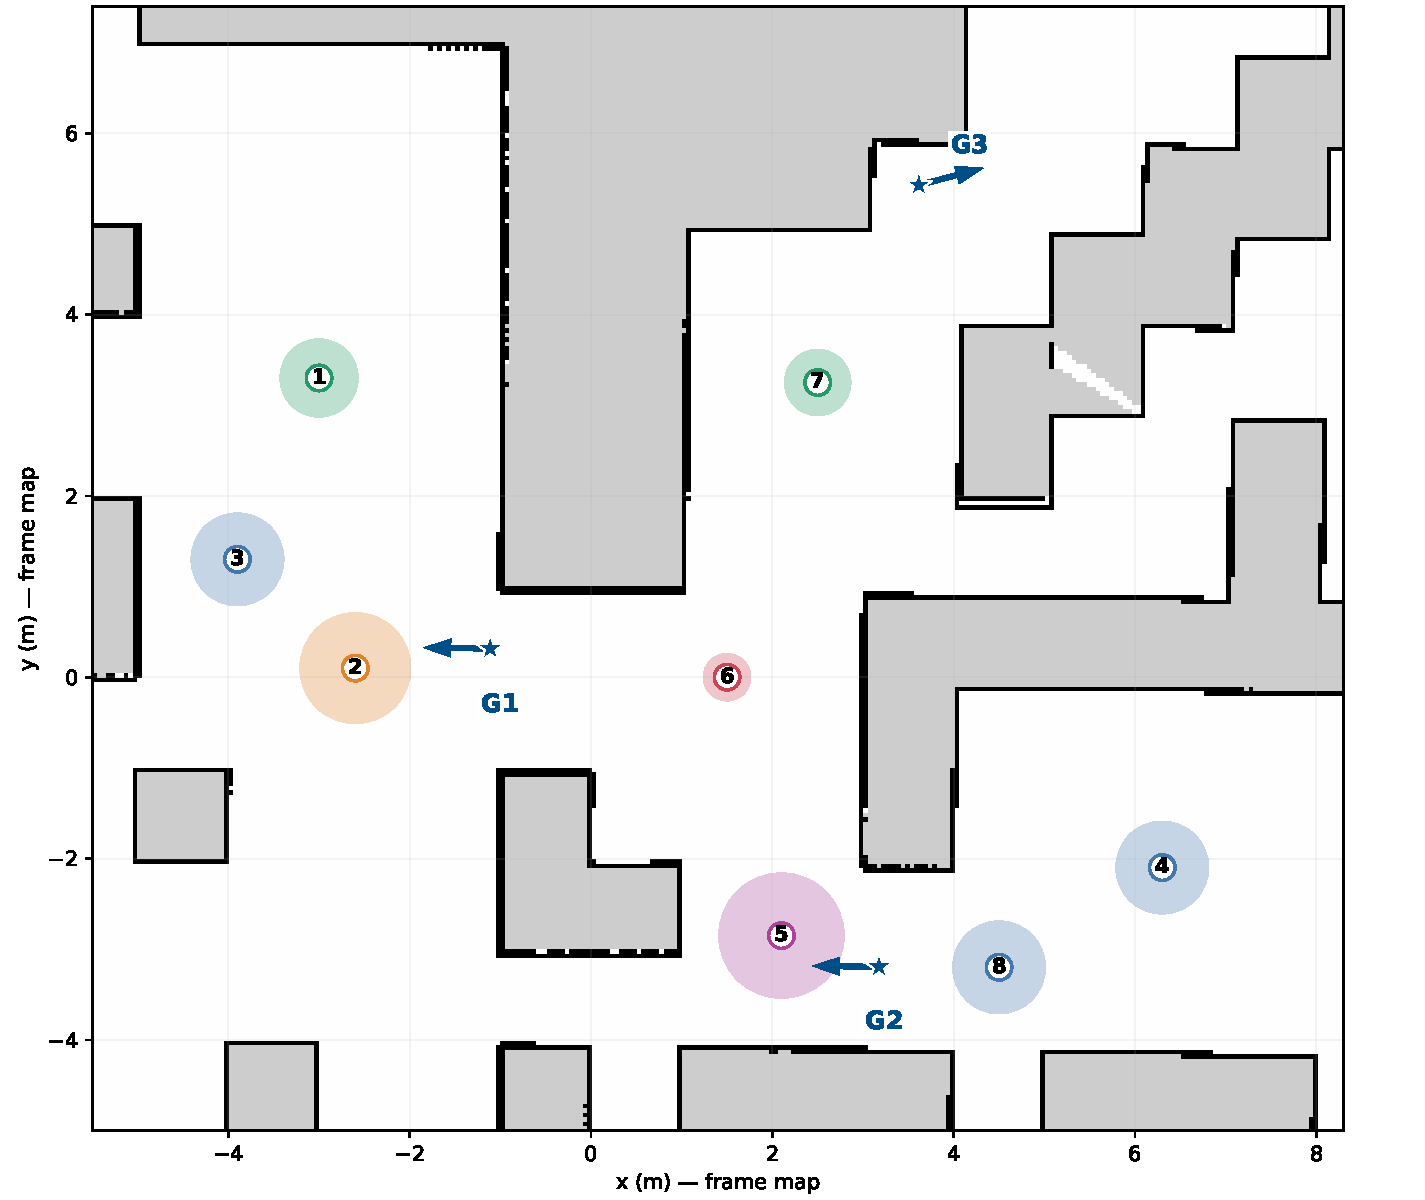
\includegraphics[width=.89\linewidth,height=10.6cm,keepaspectratio]{figures/map_goals_objects.pdf}
\caption[Map, ba goal và tám vật thể hiện tại]{Map đã lưu, ba Goal và tám vật thể hiện tại. Sao xanh chỉ goal; mũi tên chỉ yaw; đĩa màu bao footprint vật thể. Đây là sơ đồ dựng từ cấu hình và map, không phải ảnh một lần chạy mới.}\label{fig:mapgoals}
\end{figure}
\begin{table}[H]\centering\small
\caption{Tọa độ và khoảng hở tới tường maze của scene hiện tại}\label{tab:objects}
\begin{tabular}{@{}clrrrr@{}}\toprule
Số&Vật thể&$x$ (m)&$y$ (m)&Bán kính (m)&Hở tường (m)\\\midrule
1&Người&$-3.00$&3.30&0.420&1.580\\
2&Ngựa&$-2.60$&0.10&0.600&1.180\\
3&Ghế 1&$-3.90$&1.30&0.500&0.600\\
4&Ghế 2&6.30&$-2.10$&0.500&1.400\\
5&Xe đạp&2.10&$-2.85$&0.680&0.420\\
6&Trụ cứu hỏa&1.50&0.00&0.250&0.868\\
7&Cây sồi&2.50&3.25&0.354&1.146\\
8&Ghế 3&4.50&$-3.20$&0.500&0.443\\\bottomrule
\end{tabular}\end{table}
\code{check_scene.py} kiểm tra đĩa bao toàn thân với known-free map, kể cả unknown/biên ảnh, box tường SDF có transform và khoảng hở từng cặp. Ngưỡng yêu cầu là 0.35 m với tường/vùng không trống và 0.60 m giữa vật thể. Cả tám vị trí đạt kiểm tra ngày 20/10/2026; khoảng hở nhỏ nhất trên map khoảng 0.385 m và với tường thật khoảng 0.420 m, đều ở xe đạp.

SDF giữ visual/texture asset gốc, chuyển đường dẫn texture sang cache cục bộ, áp scale rồi thay collision mesh bằng box. Balô và biển STOP nằm trong danh sách retired. Kiểm tra footprint/collision box không chứng minh mọi đỉnh mesh hiển thị đều nằm trong đĩa bao hoặc mọi quỹ đạo sau này đều đi được; cần quan sát visual và chạy lại scene mới khi đánh giá thực nghiệm.
